\documentclass{article}
\usepackage{polski}
\usepackage[utf8]{inputenc}
\usepackage{graphicx}
\usepackage{tabto}
%s\usepackage[margin=2.5cm]{geomtry}

\usepackage[section]{placeins}
\usepackage{graphicx}    % Pakiet pozwalający ,,wklejać'' grafikę...
\usepackage{subcaption}
\usepackage{amsmath,amssymb,amsfonts,amsthm,mathtools}
                               % Dołączamy zestaw różnych przydatnych znaczków ...
\DeclareMathOperator{\arccosh}{arccosh}
% dane autora
\author{Wiktor Pilarczyk}
\title{Warsztaty - L3 - SK\\\large{Prowadzący: Tomasz Wierzbicki}}
\date{\today}
% początek dokumentu
\begin{document}
\maketitle
\section{Wstępna konfiguracja sieci}
\subsection{Ustawienia virtualbox'a}
W VirtualBox'ie stworzyłem 5 maszyn wirtualnych z ustawieniami sieci:\\
\tabto{0.4cm}Virbian1:\\
\tabto{0.8cm}    Adapter 1 - Internal Network - local0
\tabto{0.4cm}Virbian2:\\
\tabto{0.8cm}    Adapter 1 - Internal Network - local0
\tabto{0.8cm}    Adapter 2 - Internal Network - local1
\tabto{0.8cm}    Adapter 3 - Internal Network - local2
\tabto{0.4cm}Virbian3:\\
\tabto{0.8cm}    Adapter 1 - Internal Network - local1
\tabto{0.8cm}    Adapter 2 - Internal Network - local3
\tabto{0.4cm}Virbian4:\\
\tabto{0.8cm}    Adapter 1 - Internal Network - local2
\tabto{0.8cm}    Adapter 2 - Internal Network - local3
\tabto{0.8cm}    Adapter 3 - Internal Network - local4
\tabto{0.4cm}Virbian5:\\
\tabto{0.8cm}    Adapter 1 - Internal Network - local4\newpage
\subsection{Ustawienia sieci}
Komendy użyte do konfiguracji sieci dla poszczególnej maszyny wirtualnej (po wcześniejszym sprawdzeniu adresów MAC w ustawieniach i interfejsów za pomocą 'ip link'):
\tabto{0.4cm}Virbian1:
\tabto{0.8cm}    sudo ip link set enp0s3 name enp-loc0
\tabto{0.8cm}    sudo ip link set up dev enp-loc0
\tabto{0.8cm}    sudo ip addr add dev enp-loc0 192.168.0.1/24
\tabto{0.4cm}Virbian2:
\tabto{0.8cm}    sudo ip link set enp0s3 name enp-loc0
\tabto{0.8cm}    sudo ip link set enp0s8 name enp-loc1
\tabto{0.8cm}    sudo ip link set enp0s9 name enp-loc2
\tabto{0.8cm}    sudo ip link set up dev enp-loc0
\tabto{0.8cm}    sudo ip link set up dev enp-loc1
\tabto{0.8cm}    sudo ip link set up dev enp-loc2
\tabto{0.8cm}    sudo ip addr add dev enp-loc0 192.168.0.2/24
\tabto{0.8cm}    sudo ip addr add dev enp-loc1 192.168.1.2/24
\tabto{0.8cm}    sudo ip addr add dev enp-loc2 192.168.2.2/24
\tabto{0.4cm}Virbian3:
\tabto{0.8cm}    sudo ip link set enp0s3 name enp-loc1
\tabto{0.8cm}    sudo ip link set enp0s8 name enp-loc3
\tabto{0.8cm}    sudo ip link set up dev enp-loc1
\tabto{0.8cm}    sudo ip link set up dev enp-loc3
\tabto{0.8cm}    sudo ip addr add dev enp-loc1 192.168.1.3/24
\tabto{0.8cm}    sudo ip addr add dev enp-loc3 192.168.3.3/24
\tabto{0.4cm}Virbian4:
\tabto{0.8cm}    sudo ip link set enp0s3 name enp-loc2
\tabto{0.8cm}    sudo ip link set enp0s8 name enp-loc3
\tabto{0.8cm}    sudo ip link set enp0s9 name enp-loc4
\tabto{0.8cm}    sudo ip link set up dev enp-loc2
\tabto{0.8cm}    sudo ip link set up dev enp-loc3
\tabto{0.8cm}    sudo ip link set up dev enp-loc4
\tabto{0.8cm}    sudo ip addr add dev enp-loc2 192.168.2.4/24
\tabto{0.8cm}    sudo ip addr add dev enp-loc3 192.168.3.4/24
\tabto{0.8cm}    sudo ip addr add dev enp-loc4 192.168.4.4/24
\tabto{0.4cm}Virbian5:
\tabto{0.8cm}    sudo ip link set enp0s3 name enp-loc4
\tabto{0.8cm}    sudo ip link set up dev enp-loc4
\tabto{0.8cm}    sudo ip addr add dev enp-loc4 192.168.4.5/24
\subsection{Ustawianie domyślnej trasy}
Komendy użyte do ustawienia domyślnej trasy dla:
\tabto{0.4cm}Virbian1 przebiegająca przez Virbian2:
\tabto{0.8cm}    sudo ip route add default via 192.168.0.2/24
\tabto{0.4cm}Virbian5 przebiegająca przez Virbian4:
\tabto{0.8cm}    sudo ip route add default via 192.168.4.4/24
Po wszystkich insttukcjach warto sprawdzić czy nie popełniono błedu komendą 'ip addr'.
\subsection{Protokuł RIP}
Włączenie protokołu RIP dla Virbian2:
\tabto{0.8cm}    sudo touch /etc/quagga/ripd.conf
\tabto{0.8cm}    sudo touch /etc/quagga/zebra.conf
\tabto{0.8cm}    sudo touch /etc/quagga/vtysh.conf
\tabto{0.8cm}    sudo systemctl start ripd
\tabto{0.8cm}    sudo vtysh
\tabto{0.8cm}    configure terminal
\tabto{0.8cm}    router rip
\tabto{0.8cm}    version 2
\tabto{0.8cm}    network 192.168.0.0/24
\tabto{0.8cm}    network 192.168.1.0/24
\tabto{0.8cm}    network 192.168.2.0/24
\tabto{0.8cm}    end
\tabto{0.8cm}    exit
\tabto{0.8cm}    ip route\\
Instrukcje dla innych różnią się pomiędzy instrkucją 'version 2', a 'end' dla:
\tabto{0.4cm}Virbian3:
\tabto{0.8cm}    network 192.168.1.0/24
\tabto{0.8cm}    network 192.168.3.0/24
\tabto{0.4cm}Virbian4:
\tabto{0.8cm}    network 192.168.2.0/24
\tabto{0.8cm}    network 192.168.3.0/24
\tabto{0.8cm}    network 192.168.4.0/24
\newpage
Otrzymane tablice:

\begin{figure}[!htb]
\centering
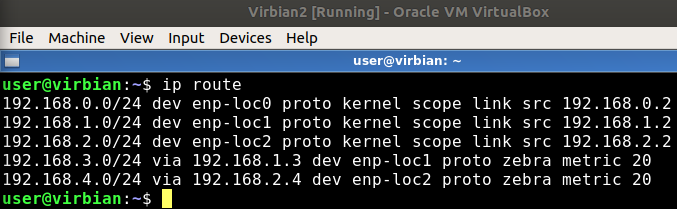
\includegraphics[width=11cm,height=3.91cm]{rout2.png}
\caption{Tablica routingu dla V2}
\end{figure}
\begin{figure}[!htb]
\centering
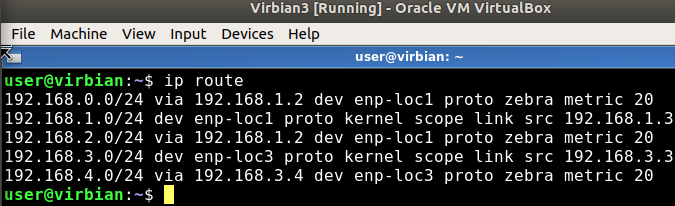
\includegraphics[width=11cm,height=3.91cm]{rout3.png}
\caption{Tablica routingu dla V2}
\end{figure}
\begin{figure}[!htb]
\centering
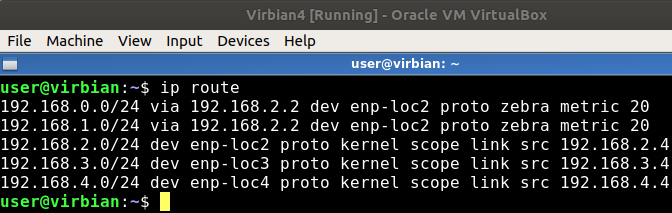
\includegraphics[width=11cm,height=3.91cm]{rout4.png}
\caption{Tablica routingu dla V4}
\end{figure}

\newpage
\section{Testowanie rozwiązania}
\begin{figure}[!htb]
\centering
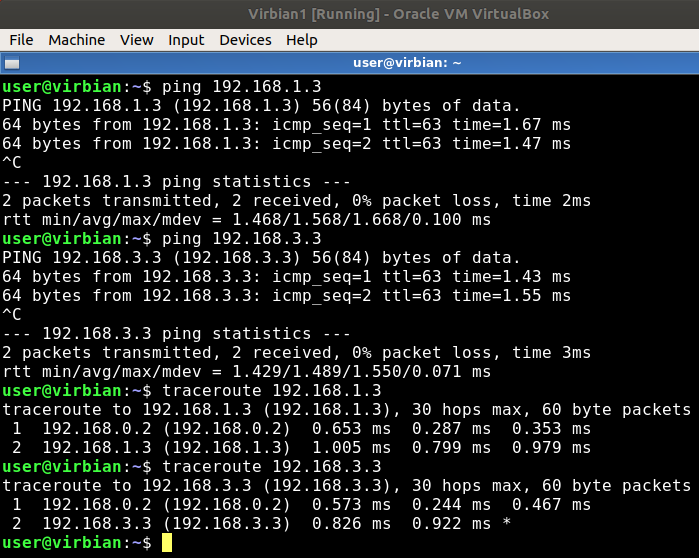
\includegraphics[width=11cm,height=7.91cm]{v11.png}
\caption{Ping i traceroute dla V1 do V3}
\end{figure}
\begin{figure}[!htb]
\centering
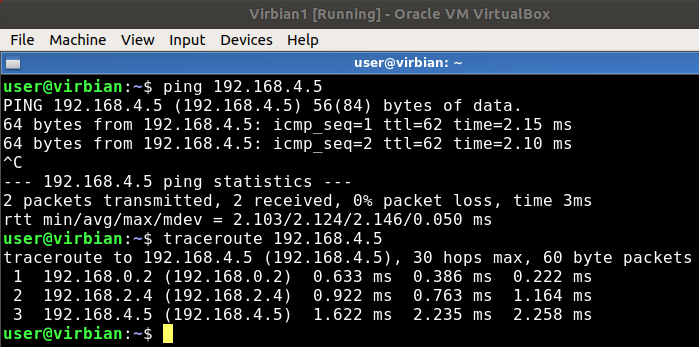
\includegraphics[width=11cm,height=4.91cm]{v12.png}
\caption{Ping i traceroute dla V1 do V2}
\end{figure}

\begin{figure}[!htb]
\centering
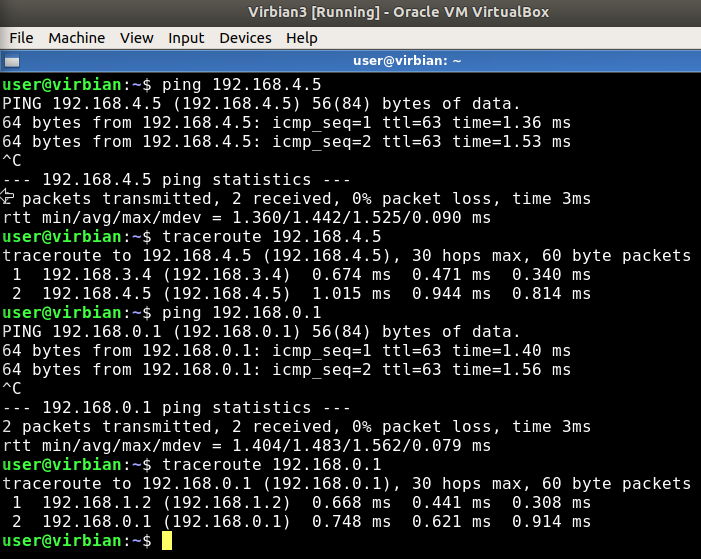
\includegraphics[width=11cm,height=4.91cm]{v3.png}
\caption{Ping i traceroute dla V3 do V1 i V5}
\end{figure}


\begin{figure}[!htb]
\centering
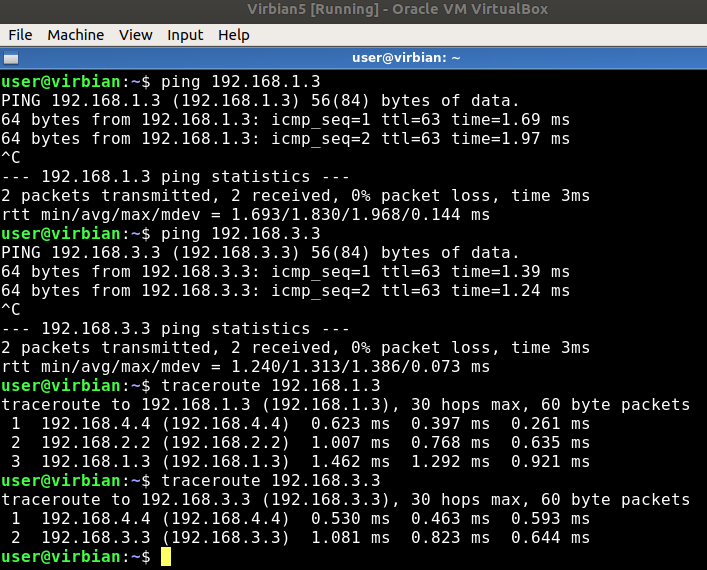
\includegraphics[width=11cm,height=7.91cm]{v51.png}
\caption{Ping i traceroute dla V5 do V3}
\end{figure}
\begin{figure}[!htb]
\centering
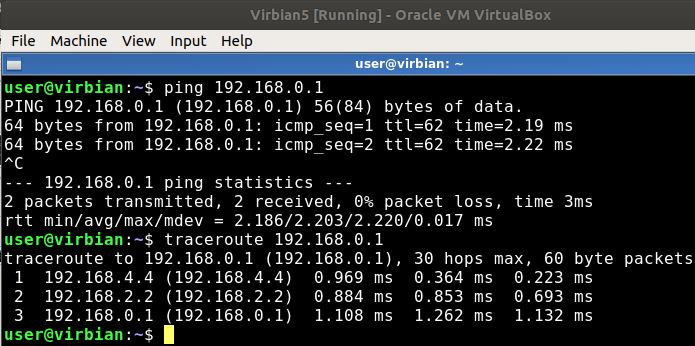
\includegraphics[width=11cm,height=4.91cm]{v52.png}
\caption{Ping i traceroute dla V5 do V1}
\end{figure}
\end{document}
